\documentclass[journal, 10pt]{IEEEtran}

\usepackage[pdftex]{graphicx}
\graphicspath{{./images/}}
\DeclareGraphicsExtensions{.pdf,.jpeg,.png}

\usepackage[cmex10]{amsmath}
\usepackage{array}

\usepackage[caption=false,font=footnotesize]{subfig}



\usepackage{url}
\usepackage[utf8x]{inputenc}
\usepackage{wasysym}
\usepackage{multirow}
\usepackage{slashbox}
\usepackage{color}
\usepackage[usenames,dvipsnames,svgnames,table]{xcolor}

\pdfminorversion=5


\def\ta{Timed Automaton}
\def\tas{Timed Automata}

\hyphenation{chan-ging}



\begin{document}

\title{Modelling biological pathway dynamics\\with \tas}


\author{
\IEEEauthorblockN{
Stefano Schivo\IEEEauthorrefmark{1},
Jetse Scholma\IEEEauthorrefmark{1},
Brend Wanders,
Ricardo A. Urquidi Camacho,\\
Paul E. van der Vet,
Marcel Karperien,
Rom Langerak,
Jaco van de Pol and
Janine N. Post
}%
\thanks{\IEEEauthorrefmark{1}These authors contributed equally to this work.}%
\thanks{S. Schivo, R. Langerak and J. van de Pol are with the Formal Methods and Tools group,
Faculty of EEMCS, University of Twente, Enschede, The Netherlands.

J. Scholma, R. A. Urquidi Camacho, M. Karperien and J. N. Post are with the Developmental BioEngineering group,
MIRA Institute for Biomedical Technology and Technical Medicine, Enschede, The Netherlands.

B. Wanders and P. E. van der Vet are with the Human Media Interaction group,
Faculty of EEMCS, University of Twente, Enschede, The Netherlands.

We acknowledge support from Netherlands Organisation for Scientific Research (NWO) CASIMIR to J.S.}%
}

\maketitle


\begin{abstract}
Living cells are constantly subjected to a plethora of environmental stimuli that require integration into an appropriate cellular response. 
This integration takes place through signal transduction events that form tightly interconnected networks. The understanding of these networks requires
to capture their dynamics through computational support and models.
ANIMO (Analysis of Networks with Interactive MOdelling) is a tool that enables construction and exploration of executable models 
of biological networks, helping to derive hypotheses and to plan wet-lab experiments.
The tool is based on the formalism of \tas, which can be analysed via
the UPPAAL model checker.
Thanks to \tas, we can provide a formal semantics for the domain-specific language used to represent signalling networks.
This enforces precision and uniformity in the definition of signalling pathways,
contributing to the integration of isolated signalling events into complex network models.
We propose an approach to discretization of reaction kinetics that allows us to efficiently use UPPAAL
as the computational engine to explore the dynamic behaviour of the network of interest.
A user-friendly interface hides the use of \tas\ from the user, while keeping the expressive power intact. 
Abstraction to single-parameter kinetics speeds up construction of models
that remain faithful enough to provide meaningful insight. The resulting dynamic behaviour of the network components 
is displayed graphically, allowing for an intuitive and interactive modelling experience.
\end{abstract}

\begin{IEEEkeywords}
 timed automata; signalling pathway; modelling; dynamic behaviour
\end{IEEEkeywords}

\IEEEpeerreviewmaketitle


\section{Introduction}\label{sec:introduction}

Systems biology aims at understanding biological systems from a holistic rather than a reductionist perspective.
As the complexity of dynamic molecular interaction networks exceeds the capacity of the human mind, 
computational support is needed to describe and understand such networks.
Large volumes of data are particularly useful when used as reference for functional models
that formalize the interactions between the components of a network.
Such models can assist in exploration and transfer of knowledge. 
Functional disease models can be combined with patient-specific expression profiles to stratify 
patients into treatment groups and maximize efficacy.

Executable biology is a relatively new area in systems biology and takes the approach of \emph{in silico} mimicking biological processes of interacting 
network components. This paradigm offers a close match with biological intuition~\cite{ex-bio}.
ODEs (ordinary differential equations) are often used to model the dynamics of biochemical processes,
and the availability of supporting tools~\cite{copasi,gna,e-cell} makes their power accessible to end users.
Process calculi are also classified as executable approaches, and tools based on such formalisms have been successfully
used in modelling complex biological events~\cite{biopepa-nfkb,blenx-parkinson}.
However, most of the existing modelling tools require theoretical foundations or training in mathematics,
and this may hamper the widespread creation of \emph{in silico} models within the biological community.
For this reason, we developed a modelling tool centred around user-friendliness, ANIMO~\cite{animo-site}, the technical foundations of which are described 
in detail in this paper. The formalism of \tas~\cite{timed-automata-alur} provides an excellent starting point for 
construction of executable models of biological networks and enables the use of the dedicated model checking tool UPPAAL~\cite{uppaal}.
The use of \tas\ to model molecular interactions has been explored before~\cite{bartocci-oscillators,ta-siebert,oded-ta-discretization}, and is further elaborated by us 
and for the first time applied in a mature modelling tool. ANIMO is implemented as a plug-in to the 
network visualization tool Cytoscape~\cite{cytoscape}, which contributes to the user friendliness and widens ANIMO's 
applicability within the biological community. The modelling process is entirely performed via the user interface, and user input is 
automatically translated into an underlying \tas\ model.

This paper extends on the BIBE conference paper presented in 2012~\cite{animo-bibe}. In the present work, we describe in detail how 
\tas\ guards and invariants are calculated from kinetic reaction equations and how unwanted side effects of rounding 
to integer time units are dealt with. Furthermore, we show how the use of UPPAAL's statistical model checker~\cite{uppaal-smc} improves simulation 
performance. Finally, a newly implemented feature is presented that assists in understanding the effect of 
modifications to the model, by using a heatmap that shows the dynamic per-node differences between two versions of the model. 
To exemplify this new functionality, we provide an illustrative case study that shows the added value for performing \emph{in silico} experiments.

After a brief introduction on the basic aspects of biological signalling networks and
\tas\ in Section~\ref{sec:preliminari}, we will explain in Section~\ref{sec:modeling-signaling-pathways} how our modelling approach works,
showing an example application in Section~\ref{sec:case-study}. After discussing related work in Section~\ref{sec:related-work},
Section~\ref{sec:conclusions} concludes the paper and gives some perspectives for future developments.


\def\ta{TA}
\def\tas{TA}

\section{Preliminaries}\label{sec:preliminari}

\subsection{Signalling pathways in biology}\label{sec:biologia}
Intra-cellular signalling pathways represent the cellular events occurring when receptors are activated by specific ligands.
A typical interaction occurring in a signalling pathway involves an upstream protein inducing a post-translational
modification (e.g. phosphorylation) to a downstream substrate. Changing the state of a protein often results in a change in its activity. 
A cascade of activating reactions relays incoming signals to their downstream targets. Graphical representations of a signalling pathway typically depict
proteins as nodes and reactions as edges, with $\rightarrow$ and $\dashv$ representing activation and inhibition, 
respectively.


Many nodes are shared by different signalling pathways and this crosstalk ties pathways into strongly interconnected 
networks that also contain feedback loops. However, the function of these networks does not only derive from their 
topology, but also from their dynamic behaviour, which cannot be deduced from traditional static representations.
This is an incentive towards a method for enriching these representations with a formal description 
of the associated dynamics. Computational models of such complex, dynamic networks would enable {\it in silico} 
experiments, generation of hypotheses and rational design of wet-lab experiments.


\subsection{Timed Automata}\label{sec:TA}
Timed Automata (\tas)~\cite{timed-automata-alur} are finite-state automata to which real-valued clocks
and communication channels have been added. In particular, clocks are used to define conditions enabling
transitions between locations of an automaton, or to limit the permanence in locations. These conditions are
called \emph{guards} and \emph{invariants}, respectively. Performing a transition may require two automata
to interact via \emph{synchronization}, where each participant performs one of two complementary actions (termed \emph{input} and \emph{output})
on a shared communication channel. Such channels can also be defined as \emph{broadcast}, allowing multi-part
communication with one sender and many receivers.
In order to obtain answers to interesting questions about the behaviour of a model, model checking~\cite{model-checking} can be applied to a \tas\ model,
using a software tool such as UPPAAL~\cite{uppaal}.

As an example of TA, a basic model of a generic signalling network is given in Figure~\ref{fig:small-example-model}.
The model represents the active fraction (further called \emph{activity level}, or simply \emph{activity} when
not ambiguous) of a population of molecules as an integer variable ({\sf reactant}, Fig.~\ref{fig:small-example-model-reactant}),
the value of which is increased (Fig.~\ref{fig:small-example-model-activation}) or decreased
by reactions. In the example, the value of {\sf reactant} is limited to 
the interval~$[0, \mbox{\sf MAX}]$, and reaching a bound may cause disabling of a reaction
(location {\sf NotReacting} in Fig.~\ref{fig:small-example-model-activation}).
More precise models of signalling networks also take into account the activity of upstream components 
when determining the availability of an activating reaction. This will be explained in the next section.

\def\taScalea{0.3}
\def\taScaleb{0.12}

\begin{figure}[htb]
\begin{center}
\subfloat[Reactant\label{fig:small-example-model-reactant}]{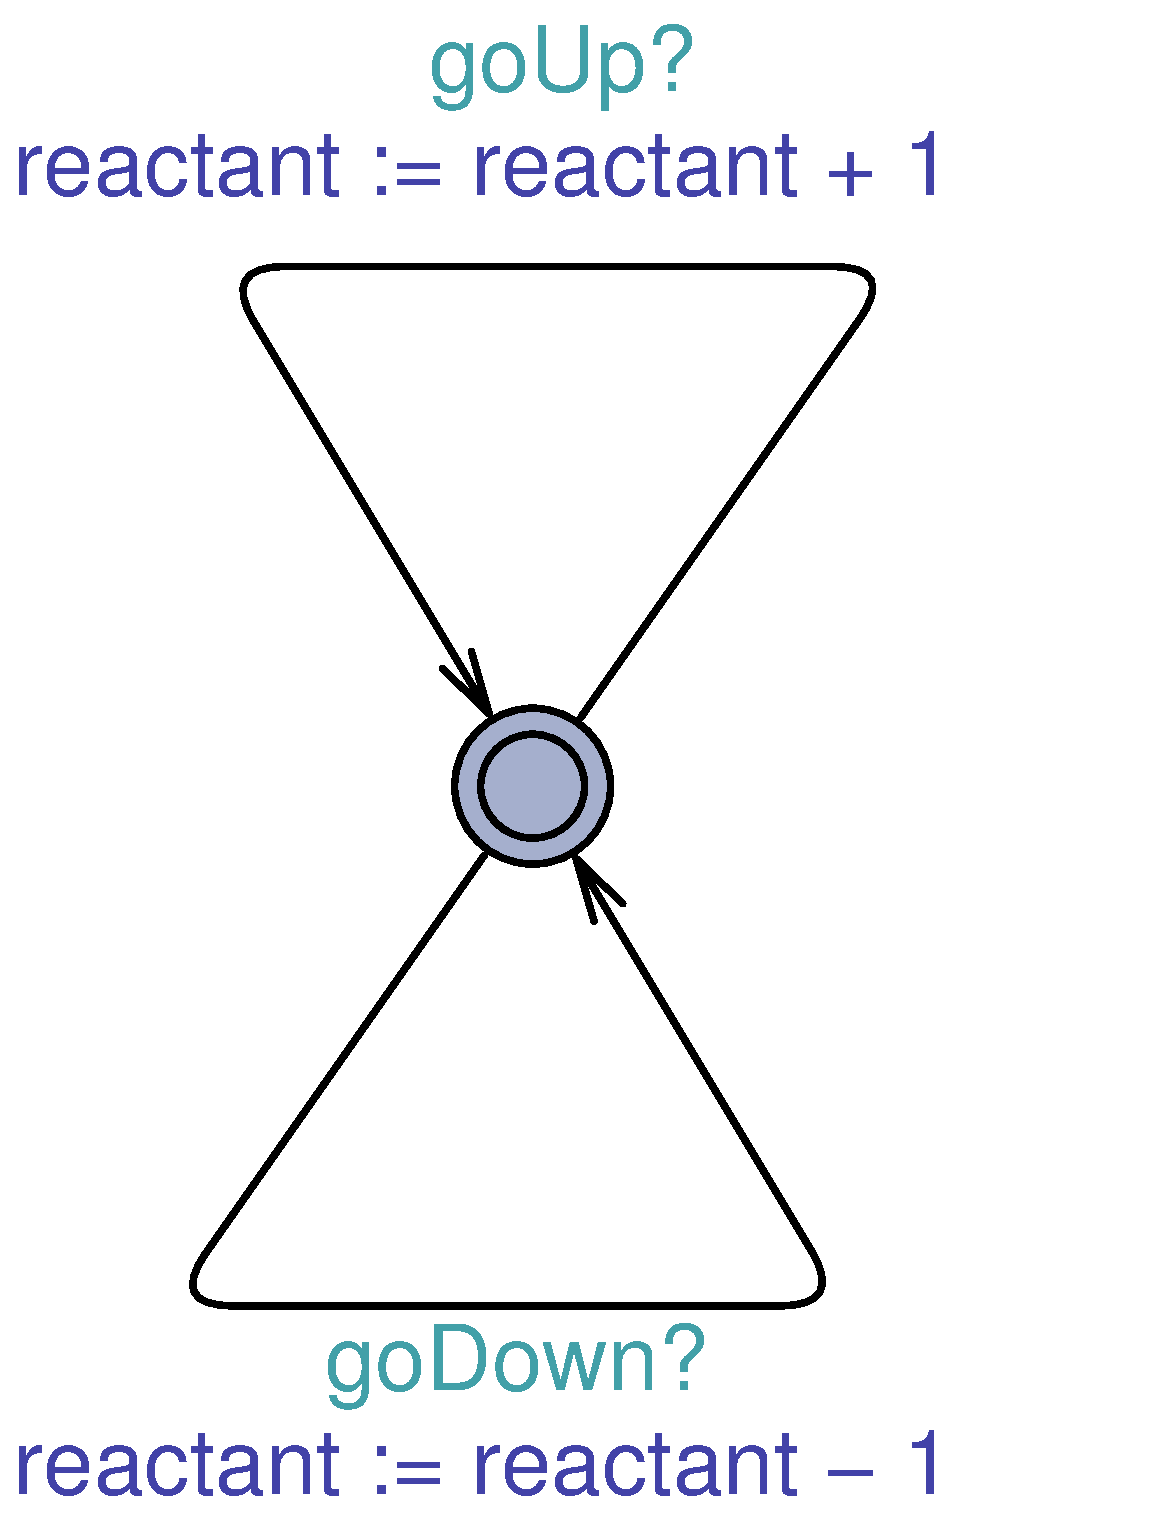
\includegraphics[scale=\taScaleb]{esempio_biologico_reactant}}\quad
\subfloat[Activation\label{fig:small-example-model-activation}]{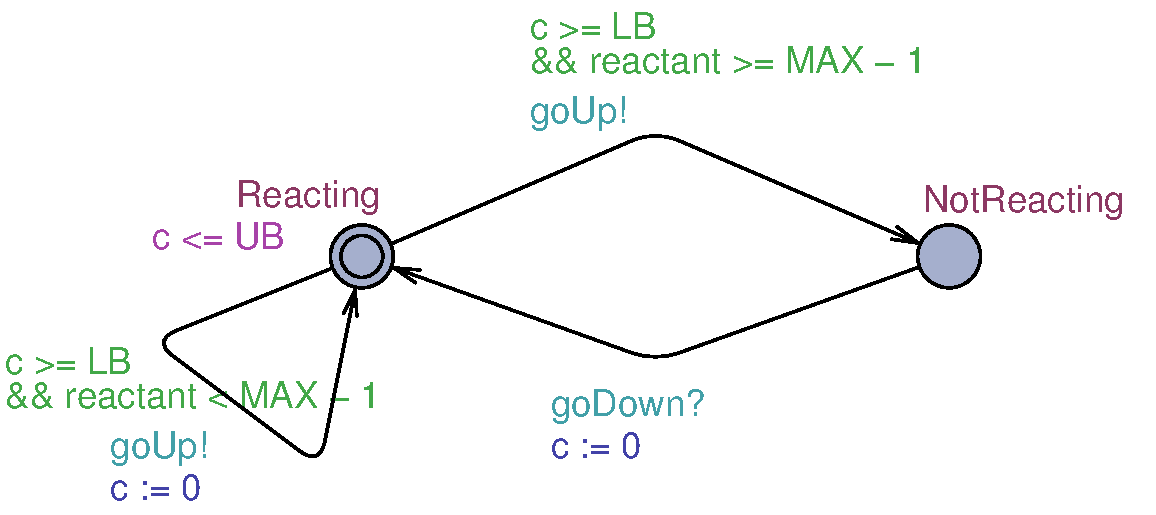
\includegraphics[scale=\taScalea]{esempio_biologico_activation}}
\caption{\tas\ templates to model a signalling pathway as represented by UPPAAL's user interface.
Each automaton starts evolving from the location marked with two concentric circles.
\protect\subref{fig:small-example-model-reactant} This automaton updates the {\sf reactant} variable
whenever a reaction occurs, changing its activity level ({\sf reactant := reactant+1} increases the activity).
\protect\subref{fig:small-example-model-activation} Activating reaction, which occurs when its internal clock {\sf c}
is inside the interval [{\sf LB, UB}] (guard $\mbox{\sf c} >= \mbox{\sf LB}$ 
and invariant $\mbox{\sf c} <= \mbox{\sf UB}$), making the target reactant's activity level increase. The current value of
{\sf reactant} ($>= \mbox{\sf MAX}-\mbox{\sf 1}$ or $< \mbox{\sf MAX}-\mbox{\sf 1}$)
determines whether the automaton takes the upper transition or the transition at the lower left.
The former ends in location {\sf NotReacting} and disables the reaction because the reactant has reached its maximum activity. The latter ends in 
location {\sf Reacting} and the reaction remains active.
An inhibiting reaction can be defined in a similar way, with the effect of decreasing the reactant's activity.
Shared broadcast channels {\sf goUp} and {\sf goDown} are used for communication between reaction and reactant automata.}
\label{fig:small-example-model}
\end{center}
\end{figure}


\section{Modelling signalling pathways}\label{sec:modeling-signaling-pathways}
\subsection{Abstraction and discretization}\label{sec:abstraction}
In order to provide experimental biologists with an intuitive way to formalize prior knowledge and experimental results,
a key aspect is to choose a suitable abstraction level.


The first abstraction made in ANIMO is the representation of 
proteins in the network in terms of their activity. Distinct biological processes can lead to activation or inhibition of proteins. 
In ANIMO, these processes are all abstracted to reactions that change the activity of downstream reactants. 

Second, we abstract from detailed elementary reactions. This is particularly useful in 
biology, where the construction of very detailed models is often hampered by 
a lack of knowledge about the exact details of the molecular mechanisms involved. 
Detailed representations of biological systems require detailed knowledge of reaction mechanisms as well as 
accompanying kinetic parameters for each individual step in the overall reaction. 
By choosing a higher abstraction level, elementary reaction steps can be aggregated into a single step in the model, reducing
the number of parameters in the model. As such, this abstraction not only reduces the time to construct a model, it also facilitates the modelling of larger networks
for which not all details of elementary reactions are known. 
Of course, a higher abstraction level also comes at the price of losing some descriptiveness, but we will demonstrate
in Section~\ref{sec:case-study} that abstracted models can capture experimental data in a meaningful way.

A third level of abstraction is the discretization of activities into integer variables with a user-defined granularity, ranging from Boolean (2 levels) 
to almost continuous (100 levels). This discretization gives the user the flexibility to adjust the model abstraction to the level of 
prior knowledge, to the quality and nature of experimental data and to the biological questions at hand. It also allows 
control over the trade-off between level of detail and computational performance for large models.


\subsection{Reaction kinetics}\label{sec:modeling-framework}
Reaction rates depend on the current activity levels of the involved reactants. For instance, a higher activity of upstream enzyme and/or a higher abundance of 
downstream substrate increase the reaction rate. 

Different degrees of complexity are taken into account when defining reaction kinetics. Given a reaction in which $A$ (enzyme) activates $B$ (substrate), we define $R$ as the time needed to increase the activity level of $B$ by 1. $R$ is computed using a kinetic function $f$ that
depends on the current activity levels of both $A$ and $B$: $R = f(a, b)$

$$
f(a, b) = \left\{ \begin{array}{ll}
		      \frac{1}{r(a, b)} \times \mbox{\it levelsScale} \times \mbox{\it timeScale} & \mbox{ if } r(a, b) \neq 0 \\
		      \infty & \mbox{ otherwise}
                  \end{array} \right.
$$


The reaction rate $r$ is computed from a single kinetic constant $k$ and the activity levels of the reactants. Three kinetic scenarios are implemented :\\
%\begin{description}
{\bf Scenario 1}: $r(a) = k \times a$ : the reaction rate depends on the activity level of the upstream enzyme only. \\
{\bf Scenario 2}: $r(a, b) = k \times a \times b$ : the reaction rate depends on the activity levels of both the upstream enzyme and the
downstream substrate. $b$ represents the inactive fraction of substrate if the reaction
is an activation, whereas it refers to the active fraction when the effect is inhibitory.\\
{\bf Scenario 3}: $r(c, d) = k \times c \times d$ : the reaction rate depends on the activity of two upstream components chosen by the user. This scenario performs a function analogous to an AND-gate in Boolean models.

{\it levelsScale} is a scale factor that allows to keep reaction kinetics independent from the granularity of its reactants. 
The value of {\it levelsScale} depends on the kinetic scenario used to compute $r$. With $nA$ the granularity of reactant $A$
(and similarly for other reactants), {\it levelsScale} is defined as:\\
{\bf Scenario 1}: $\mbox{\it levelsScale} = \frac{nA}{nB}$\\[1ex]
{\bf Scenario 2}: $\mbox{\it levelsScale} = \frac{nA \times nB}{nB} = nA$\\[1ex]
{\bf Scenario 3}: $\mbox{\it levelsScale} = \frac{nC \times nD}{nB}$, with $nB$ the granularity of the reactant influenced by the reaction.\\
The numerators are used to normalize all input activity values to the $[0, 1]$ interval, which keeps the reaction
kinetics independent from the input reactants' granularity. The denominator works similarly on the downstream reactant.
The importance of this can be intuitively understood with a simple example.
Consider an activating reaction $A \rightarrow B$, with $A$ completely
active and $B$ completely inactive. If $B$ has $10$ granularity levels and no other reactions influence $A$ or $B$,
the reaction will take $T$ seconds to completely activate $B$ from $0$ to $10$ levels. When the granularity of $B$ would be increased to
$30$ levels, the reaction should still take $T$ seconds to completely activate $B$, bringing it
from $0$ to $30$ levels. This implies that each reaction step that increases the activity of B by one level takes one third 
of the time it took in the situation with 10 activity levels for $B$. This scaling is accounted for by using $nB$ as denominator in {\it levelsScale}.


{\it timeScale} is based on the ratio between real-life seconds and \ta\ time units. This enables performing simulation runs using
real-life units of time. Moreover, as an UPPAAL model must express all time bounds as integers,
{\it timeScale} is automatically optimized to prevent rounding problems when $R$ would be rounded to 0 for values $< 0.5$.
Increasing the value for {\it timeScale} ensures that the smallest value for $R$ becomes larger than 0.
It is important to note that {\it timeScale} cannot simply be assigned an arbitrarily high value, because  
the resulting time constraints could overflow the maximum constant allowed in UPPAAL (currently, $2^{30}-2$).
ANIMO automatically chooses the optimum {\it timeScale} value by making a preliminary
computation of all borderline values, i.e. the minimum and maximum time constraint for each reaction.
The starting value for {\it timeScale} is computed as
$$
\mbox{\it timeScale} = \frac{1}{\mbox{\it secondsPerStep}}
$$
where {\it secondsPerStep} is the user-chosen ratio between real-life seconds and \ta\ time units, with 1 as its default value.
The resulting value is then optimized (raised or lowered) to ensure that all time bounds are inside the allowed interval $[0, 2^{30}-2]$.

Finally, to take into account a natural variability that occurs in biological reactions in which reactants are 
present in low copy numbers, an uncertainty parameter can be set for each reaction.
This uncertainty is translated to time intervals for model transitions, as is shown in the model in Figure~\ref{fig:small-example-model} (cf. {\sf LB} and {\sf UB} time bounds).
With an uncertainty value of $5 \%$, the upper and lower bounds of $R$ are computed as:
$$
\begin{array}{lcl}
R(a, b)_{\mbox{\scriptsize lower bound}} &=& f(a, b) \times 0.95 \\
R(a, b)_{\mbox{\scriptsize upper bound}} &=& f(a, b) \times 1.05
\end{array}
$$
for all values of $a$ and $b$. 

As we represent activity levels $a$, $b$ via integer variables, there is a finite number of
combinations for the values of $a$ and $b$. A two-dimensional table is pre-computed, containing all possible values for $R$. 
As an example of this computation, Table~\ref{tab:lower-upper-bounds} shows the lower and upper
bounds table for a reaction $A \rightarrow B$, using scenario 2. 

\renewcommand{\tabcolsep}{2mm}
\begin{table}[htbp]
\caption{Lower and upper bounds for a reaction $A \rightarrow B$ with kinetic scenario 2, $k = 0.004$ (corresponding to the \emph{medium} preset)
and 10 seconds per UPPAAL time step. Granularity of $A$ is 5 (i.e. 5 activation steps from 0 to maximum activity), granularity of $B$ is 3. In both cases,
0 means completely inactive. With these settings, $\mbox{\it levelsScale} = 5.0$ and $\mbox{\it timeScale} = 0.1$. Uncertainty is set at $5 \%$.
{\color{BrickRed}Red} numbers are lower bounds, {\color{ForestGreen} green} numbers are upper bounds.}\label{tab:lower-upper-bounds}
\centering
    \begin{tabular}{|c||c|c|c|c|c|c|}
      \hline
      {\backslashbox[2em]{$B$\kern-2em}{\kern-1em$A$}} & \makebox[.5em]{0} & \makebox[.5em]{1} & \makebox[.5em]{2} & \makebox[.5em]{3} & \makebox[.5em]{4} & \makebox[.5em]{5} \\
      \hline\hline
      \begin{minipage}[c][1em][c]{1em}\centering 0\end{minipage} & \makebox[.5em]{$\infty$} & [{\scriptsize\color{BrickRed}40}, {\scriptsize\color{ForestGreen}44}] & [{\scriptsize\color{BrickRed}20}, {\scriptsize\color{ForestGreen}22}] & [{\scriptsize\color{BrickRed}13}, {\scriptsize\color{ForestGreen}15}] & [{\scriptsize\color{BrickRed}10}, {\scriptsize\color{ForestGreen}11}] & [{\scriptsize\color{BrickRed}8}, {\scriptsize\color{ForestGreen}9}] \\
      \hline
      \begin{minipage}[c][1em][c]{1em}\centering 1\end{minipage} & \makebox[.5em]{$\infty$} & [{\scriptsize\color{BrickRed}59}, {\scriptsize\color{ForestGreen}66}] & [{\scriptsize\color{BrickRed}30}, {\scriptsize\color{ForestGreen}33}] & [{\scriptsize\color{BrickRed}20}, {\scriptsize\color{ForestGreen}22}] & [{\scriptsize\color{BrickRed}15}, {\scriptsize\color{ForestGreen}16}] & [{\scriptsize\color{BrickRed}12}, {\scriptsize\color{ForestGreen}13}] \\
      \hline
      \begin{minipage}[c][1em][c]{1em}\centering 2\end{minipage} & \makebox[.5em]{$\infty$} & [{\scriptsize\color{BrickRed}119}, {\scriptsize\color{ForestGreen}131}] & [{\scriptsize\color{BrickRed}59}, {\scriptsize\color{ForestGreen}66}] & [{\scriptsize\color{BrickRed}40}, {\scriptsize\color{ForestGreen}44}] & [{\scriptsize\color{BrickRed}30}, {\scriptsize\color{ForestGreen}33}] & [{\scriptsize\color{BrickRed}24}, {\scriptsize\color{ForestGreen}26}] \\
      \hline
      \begin{minipage}[c][1em][c]{1em}\centering 3\end{minipage} & \makebox[.5em]{$\infty$} & $\infty$ & $\infty$ & $\infty$ & $\infty$ & $\infty$\\
      \hline
    \end{tabular}
\end{table}

The choice of the scenario and the value for the corresponding parameter $k$ are the only inputs requested when
defining the kinetics of a reaction. To further simplify the modelling process,
we implemented the possibility to use qualitative values for $k$, by providing a pre-defined set of 
reaction rates, labelled \emph{very slow}, \emph{slow}, \emph{medium}, \emph{fast}, \emph{very fast}. These options encourage
construction of a model in which relative reaction rates define the network dynamics. In subsequent steps, the preliminary model can be fit 
to experimental data by more precisely setting the values for $k$.

\subsection{Timed Automata model}\label{subsec:TA-templates}
An ANIMO network model contains an instance of the Reaction \ta\ template (Fig.~\ref{fig:reaction})
for each reaction present in the model. An integer variable is defined
for each of the $n$ reactants of the network to represent the reactant's current activity level. This variable is initialized as
specified by the user.
Finally, a series of channels called
$\mbox{\sf reacting}_i$, with $i \in \{1, 2, \dots, n\}$, is defined to allow reaction processes to communicate 
when the activity level of the $i$-th reactant has been updated.

\begin{figure}[htb]%
\centering%
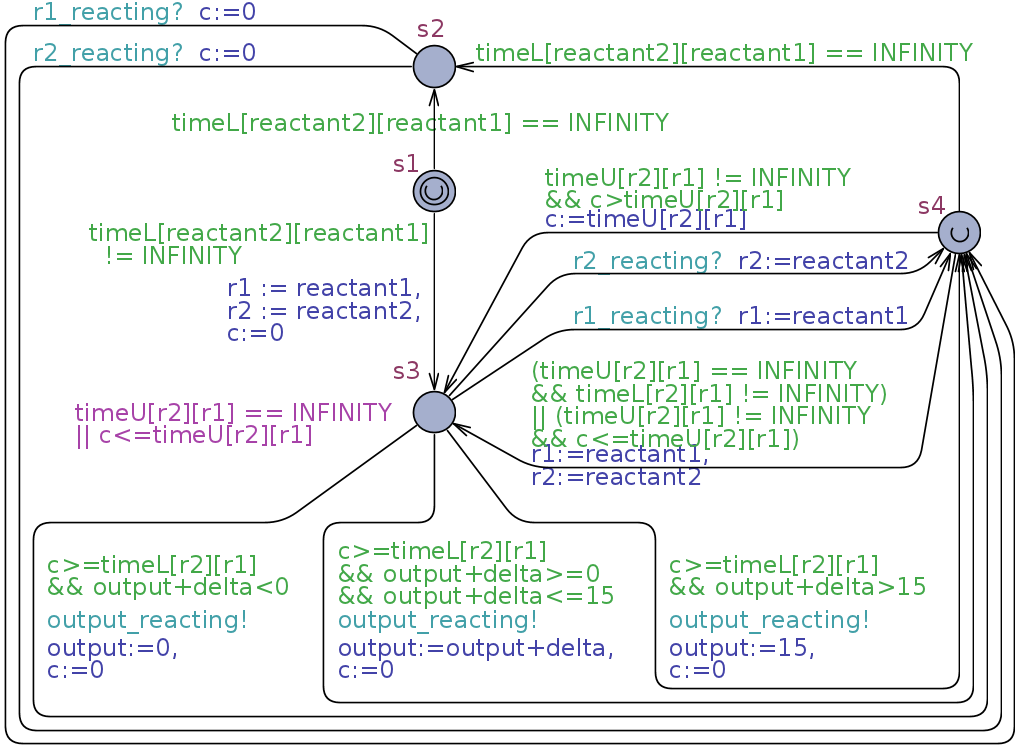
\includegraphics[width=.48\textwidth]{model_ta3}%
\caption{The \ta\ template for the reactions in the model. The two matrices {\sf timeL} and {\sf timeU} define
the lower and upper time bounds for each possible combination of the activity levels of the
reactants on which the reaction rate depends. Channels {\sf r1\_{}reacting}, {\sf r2\_{}reacting} and
{\sf output\_{}reacting} are used for communicating modifications to the value of the reactants involved.
Each of these three channels is a reference to a global shared channel {\sf reacting$_i$},
where $i$ is the index of the corresponding reactant. The output reactant is assumed
here to have 15 levels of granularity, and the guards ensure that $0 \leq \mbox{\sf output} + \mbox{\sf delta}
\leq 15$.\label{fig:reaction}}
\end{figure}

The \tas\ template in Figure~\ref{fig:reaction} depends on two input reactants, to which {\sf reactant1} and {\sf reactant2}
are references, and influences one reactant ({\sf output}). This template is used for kinetic scenarios 2 and 3, whereas
a slightly simpler template is used for scenario 1 that relies on a single input.
The basic concept underlying the Reaction \ta\ is to perform a continuous cycle, where at each iteration
 the activity level of the target reactant (variable {\sf output}) is updated upon completion of the reaction.
The variable {\sf delta} represents the increment caused in {\sf output} when the reaction occurs: thus, {\sf delta} contains
$+1$ if the reaction is an activation and $-1$ for inhibitory reactions.
The locations in the Reaction \ta\ template in Figure~\ref{fig:reaction} have been labelled {\sf s1, s2, s3, s4}, where
{\sf s1} is the starting location.


{\sf s1} is used to reset the internal clock {\sf c} and start
counting (transition to location {\sf s3}) or to enter a ``dormant'' location if the reaction cannot occur
(transition to location {\sf s2}). This is the case when the lower bound of the reaction duration
is declared as {\sf INFINITY} (i.e. the reaction rate is 0, see the definition of $f(a, b)$ in Sect.~\ref{sec:modeling-framework}). %Eq.~\ref{formula:reaction-speed}).
For instance, if the reaction activates its target and the kinetics are based on scenario 2,
the reaction cannot occur if either no inactive substrate or no active enzyme are available (cf. Tab.~\ref{tab:lower-upper-bounds}).
The {\sf U} symbol inside locations {\sf s1} and {\sf s4} marks them as \emph{urgent}:
while there is at least one automaton in an urgent location, time cannot progress. In this way,
all necessary updates are made before the reactions can continue.

The waiting location is identified by the label {\sf s3}: the automaton can exit from
this location when the activity level of an input reactant has been changed by another reaction (transitions from {\sf s3} to
{\sf s4}, receiving a communication on channel {\sf r1\_{}reacting} or {\sf r2\_{}reacting}), or when the current value
of the internal clock {\sf c} is inside the interval
$[R[\mbox{\sf r2}][\mbox{\sf r1}]_{\mbox{\scriptsize lower bound}}, R[\mbox{\sf r2}][\mbox{\sf r1}]_{\mbox{\scriptsize upper bound}}]$,
i.e. when the reaction can occur. The bounds for $R$ under the current conditions are found in the
tables {\sf timeL[\,][\,]} (corresponding to $R[\,][\,]_{\mbox{\scriptsize lower bound}}$)
and {\sf timeU[\,][\,]} ($R[\,][\,]_{\mbox{\scriptsize upper bound}}$),
which are indexed by the current activity levels of the two input reactants {\sf r1} and {\sf r2}.

If the reaction cannot occur (e.g. because all substrate is already active), the automaton stays in location {\sf s2}
until an update takes place, which can possibly change the current situation (transitions from {\sf s2} to {\sf s4}).

Finally, location {\sf s4} is used to check that the clock settings are consistent with the current time bounds.

For an example run, consider two reactions $R_1 = A \rightarrow B$ and $R_2 = C \dashv B$, both based on scenario 2, with starting
activity levels $A = 10/10$, $B = 0/10$, $C = 10/10$. The two automata for $R_1$ and $R_2$ will start
from location {\sf s1} and move immediately to {\sf s3} and {\sf s2} respectively. As 
both reactions depend on the activity level of $B$ (see the definition of scenario 2 in Sect.~\ref{sec:modeling-framework}) and
$B$ is completely inactive,
$R_1$ can proceed at full speed, while $R_2$ cannot occur. After some time (depending on the parameter $k$ of $R_1$),
transition {\sf s3} $\rightarrow$ {\sf s4} will be taken by the automaton for $R_1$, increasing the activity level
of the output reactant $B$ by 1 ({\sf output = output + delta} in the template).
At the same time, a synchronization on channel $\mbox{\sf reacting}_B$ (corresponding
to {\sf output\_{}reacting} for $R_1$ and to {\sf r2\_{}reacting} for $R_2$) will allow the automaton for $R_2$ to reach 
location {\sf s4}. $\mbox{\sf reacting}_B$
also corresponds to {\sf r2\_{}reacting} in the automaton for $R_1$,
but that automaton is already performing {\sf output\_{}reacting!}, and no more than one transition can be taken at a time.
As $R_1$ can still occur with $A = 10/10$ and $B = 1/10$, the proper {\sf s4} $\rightarrow$ {\sf s3} transition is taken next.
For the same reason, a transition {\sf s4} $\rightarrow$ {\sf s3} is taken in the automaton for $R_2$, making both reactions
active. From this point, the evolution of the system will proceed depending on the kinetic parameters defined for the reactions,
and the activity of $B$ will vary depending on which of the two reactions will occur faster, i.e. more frequently.




\subsection{Analysis with ANIMO}\label{sec:analysis-animo}

We use the statistical model checking engine~\cite{uppaal-smc} of the UPPAAL model checker to obtain a simulation run of the model. 
In order to obtain the required data, ANIMO generates a query of the form ${\tt simulate}\ 1\ [<=36000] \{ r_0, r_1, \dots, r_n \}$, 
which can be read as ``perform one simulation run until 36000 time units and produce a trace where the values of 
variables $r_0, r_1, \dots, r_n$ (the reactant activities) are shown''. This approach is considerably faster (especially in large models) 
than the one we presented previously~\cite{animo-bibe}, because only strictly needed data is produced by UPPAAL, greatly 
reducing the time needed for parsing the result. Note that the number of simulations is normally fixed to one, so 
no real statistical model checking is done when asking for one simulation. In order to see the result of multiple 
simulation runs of the same model, the user needs to select the option \emph{Compute X runs} on the ANIMO interface, 
choosing how many simulations have to be performed.
Parsed traces can be graphically explored in the ANIMO user interface, where they are displayed as time-series graphs 
of the selected reactants. In case of multiple simulation runs, the user can choose whether to obtain a plot of the averages 
(with standard deviation bars) or an overlay plot of all the computed series.
Experimental time series data can be added to the graph, enabling a direct comparison with model predictions.
By moving a slider at the bottom of the time series graph, the original input model is interactively enhanced by 
colour codings, showing the activity levels of all reactants for each time instant.

   


\section{Case study}\label{sec:case-study}
As an example application of our approach, we present a model that describes signalling events
downstream of two growth factors that regulate cell development and function in PC12 cells:
epidermal growth factor (EGF) and nerve growth factor (NGF). PC-12 cells are a model cell line to study neuronal differentiation.
We modelled part of the signalling network and compared the behaviour of our model with experimental data from Santos et al.~\cite{egf-ngf}.

It has been observed that the activation of extracellular regulated kinase (ERK) shows significantly different 
dynamics upon treatment with EGF as compared to treatment with NGF. A transient, peak-shaped 
activation is observed when PC-12 cells are treated with EGF, whereas treatment with NGF results in sustained activation of ERK,
even after removal of the input signals via growth factor-neutralizing antibodies. These activation profiles are tied to different cellular 
outcomes, with transient activation leading to proliferation and sustained activation leading to differentiation. 
These findings led the authors of~\cite{egf-ngf} to hypothesize the existence of a positive feedback from ERK to an upstream node in the network and 
existence of a new network component that blocks this feedback. It was found that NGF prevents this blocking, leading to sustained activation~\cite{egf-ngf}.
We have formalized and implemented these topological reasonings in an ANIMO model, shown in Figure~\ref{fig:case-study-model}. 
The parameters used in this network are given in Table~\ref{tab:case-study-parameters}.
The reference experimental conditions are the addition of either EGF or NGF
in sufficient quantity to fully activate their respective receptors. After 10 minutes a growth factor-neutralizing 
antibody is added, shutting off the input signal to the network. The evolution of the network is
observed for 60 minutes from the initial treatment.

\begin{figure}[htb]
\centering
  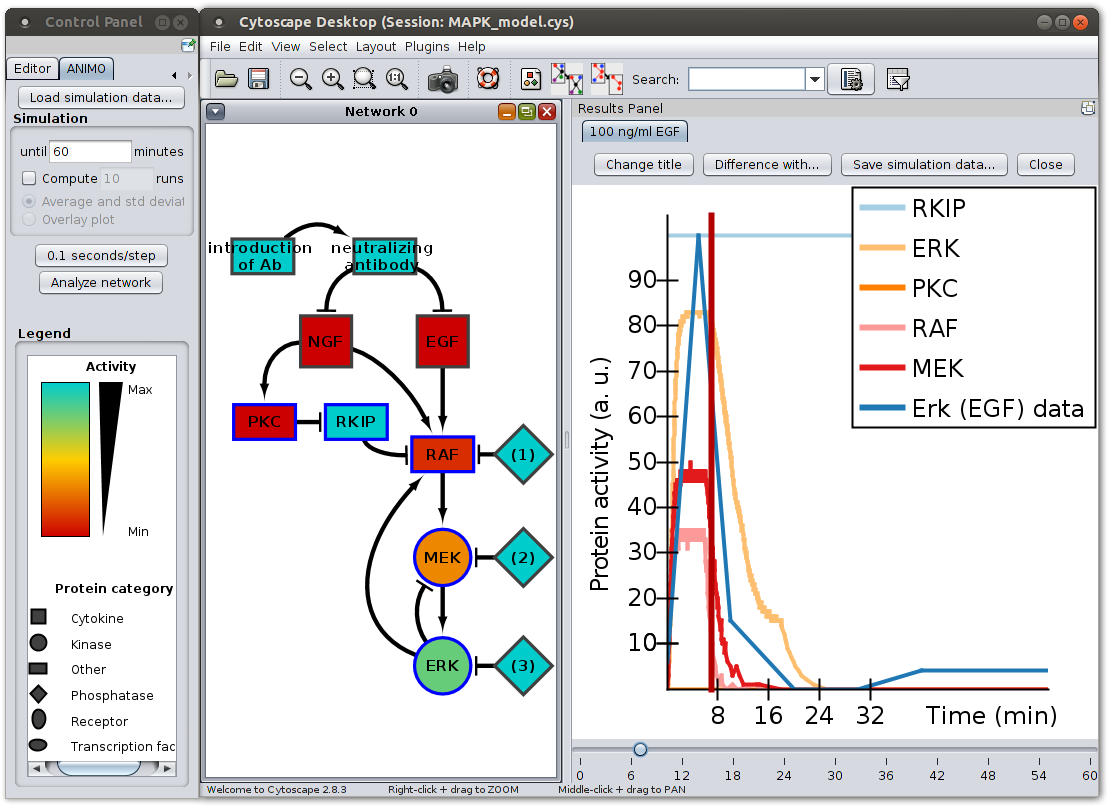
\includegraphics[width=.48\textwidth]{mapk_model_egf7}
\caption{The model represented in the ANIMO user interface.
The \emph{Network} central panel represents the model as the classical nodes-edges network
familiar in biology. To this representation, node colours and shapes are added %in order
to represent current activity levels and protein categories, as defined in the \emph{Legend}
panel on the left. On the right, the \emph{Results Panel} shows a graph of the activities
of selected nodes during the user-chosen interval of 60 minutes.
A vertical red bar, which can be moved with the underlying slider, indicates the point in
the simulation trace on which the colouring of the nodes in the \emph{Network} panel is based.
The graph allows the user to visually compare simulation results with experimental data.
The {\sf Erk (EGF) data} series is based on experimental data from Santos et al.~\cite{egf-ngf}.
}\label{fig:case-study-model}
\end{figure}


Nodes labelled as {\sf EGF}, {\sf NGF}, {\sf PKC}~(protein kinase~C),
{\sf RKIP}~(Raf kinase inhibitory protein), {\sf RAF}~(Raf), {\sf MEK}~(MAPK ERK kinase), and {\sf ERK}
in the ANIMO model correspond to the proteins in the network topology that was presented by Santos et al.~\cite{egf-ngf}.
Nodes {\sf introduction of Ab} and {\sf neutralizing antibody} are used to represent
the introduction of growth factor-neutralizing antibody after 10 minutes from the start of the initial treatment.
The reaction that activates node {\sf neutralizing antibody} takes 10 minutes to complete.
Finally, nodes labelled {\sf (1)}, {\sf (2)} and~{\sf (3)} are phosphatases that inactivate their targets. 
These inactivations cause cellular signalling networks to be reset
to their resting state after a signal has been processed. 
The feedback activation from ERK to RAF is shown as an edge from ERK to RAF in Fig.~\ref{fig:case-study-model}.
In the absence of PKC activity, RKIP is active and inhibits RAF. When PKC is activated by NGF, RKIP is phosphorylated and inhibited by PKC,
causing sustained activation of RAF by ERK (cf. Fig.~\ref{fig:ngf-graph}).

\begin{table}[htb]
\begin{center}
\caption{Parameter settings for the model in Figure~\ref{fig:case-study-model}.
The Scen. column contains the number of the kinetic scenario for each reaction (see Sect.~\ref{sec:modeling-framework}).
\ensuremath{^{(*)}} In order to reflect experimental treatment conditions, the settings for initial NGF and EGF activity
are to be considered mutually exclusive: if one is at maximum activity, the other is set at 0.}\label{tab:case-study-parameters}
\scriptsize
  \begin{tabular}{|l|l|l||l|l|l|}
   \hline
    \multicolumn{3}{|c||}{\bf Reactants} & \multicolumn{3}{c|}{\bf Reactions}\\
    \hline
    \hline
    {\bf Name} & {\bf Levels} & {\bf Init act.} & {\bf Reaction} & {\bf Scen.} & $k$\\
    \hline
    intr. Ab & 1 & 1 & intr. Ab $\rightarrow$ neutr. Ab & 1 & 0.003\\
    \hline
    neutr. Ab & 1 & 0 & neutr. Ab $\rightarrow$ NGF & 2 & 0.00375\\
    \hline
    NGF & 15 & $15^{(*)}$ & neutr. Ab $\dashv$ EGF & 2 & 0.0625\\
    \hline
    EGF & 15 & $15^{(*)}$ & NGF $\rightarrow$ PKC & 2 & 7e-4\\
    \hline
    PKC & 40 & 0 & NGF $\dashv$ RAF & 2 & 0.005\\
    \hline
    RKIP & 20 & 20 & EGF $\rightarrow$ RAF & 2 & 0.0125\\
    \hline
    RAF & 60 & 0 & PKC $\dashv$ RKIP & 2 & 0.004\\
    \hline
    (1) & 1 & 1 & RKIP $\dashv$ RAF & 2 & 0.02\\
    \hline
    MEK & 60 & 0 & (1) $\dashv$ RAF & 2 & 0.0035\\
    \hline
    (2) & 1 & 1 & ERK $\rightarrow$ RAF & 2 & 3.75e-4\\
    \hline
    ERK & 100 & 0 & RAF $\rightarrow$ MEK & 2 & 0.054\\
    \hline
    (3) & 1 & 1 & (2) $\dashv$ MEK & 2 & 0.0049\\
    \hline
     & & & ERK $\dashv$ MEK & 2 & 0.0192\\
    \hline
     & & & MEK $\rightarrow$ ERK & 2 & 0.075\\
    \hline
     & & & (3) $\dashv$ ERK & 2 & 0.0075\\
    \hline
  \end{tabular}
\end{center}
\end{table}


The dynamic behaviour of ERK in the model and from the experimental data is shown in Figure~\ref{fig:case-study-graphs}. 
The model reflects the general behaviour of ERK: transient activation results from treatment with EGF,
whereas NGF treatment causes sustained activation. In this model, we deliberately left out a number of proteins,
e.g. the receptors for EGF and NGF, since no experimental data were available for these nodes. In order to further refine the model, 
these intermediate nodes could be added to the model. In this way, the model could fit the data more closely, 
going beyond the scope of this example.


\begin{figure}[htb]
\centering
\subfloat[\label{fig:egf-graph}]{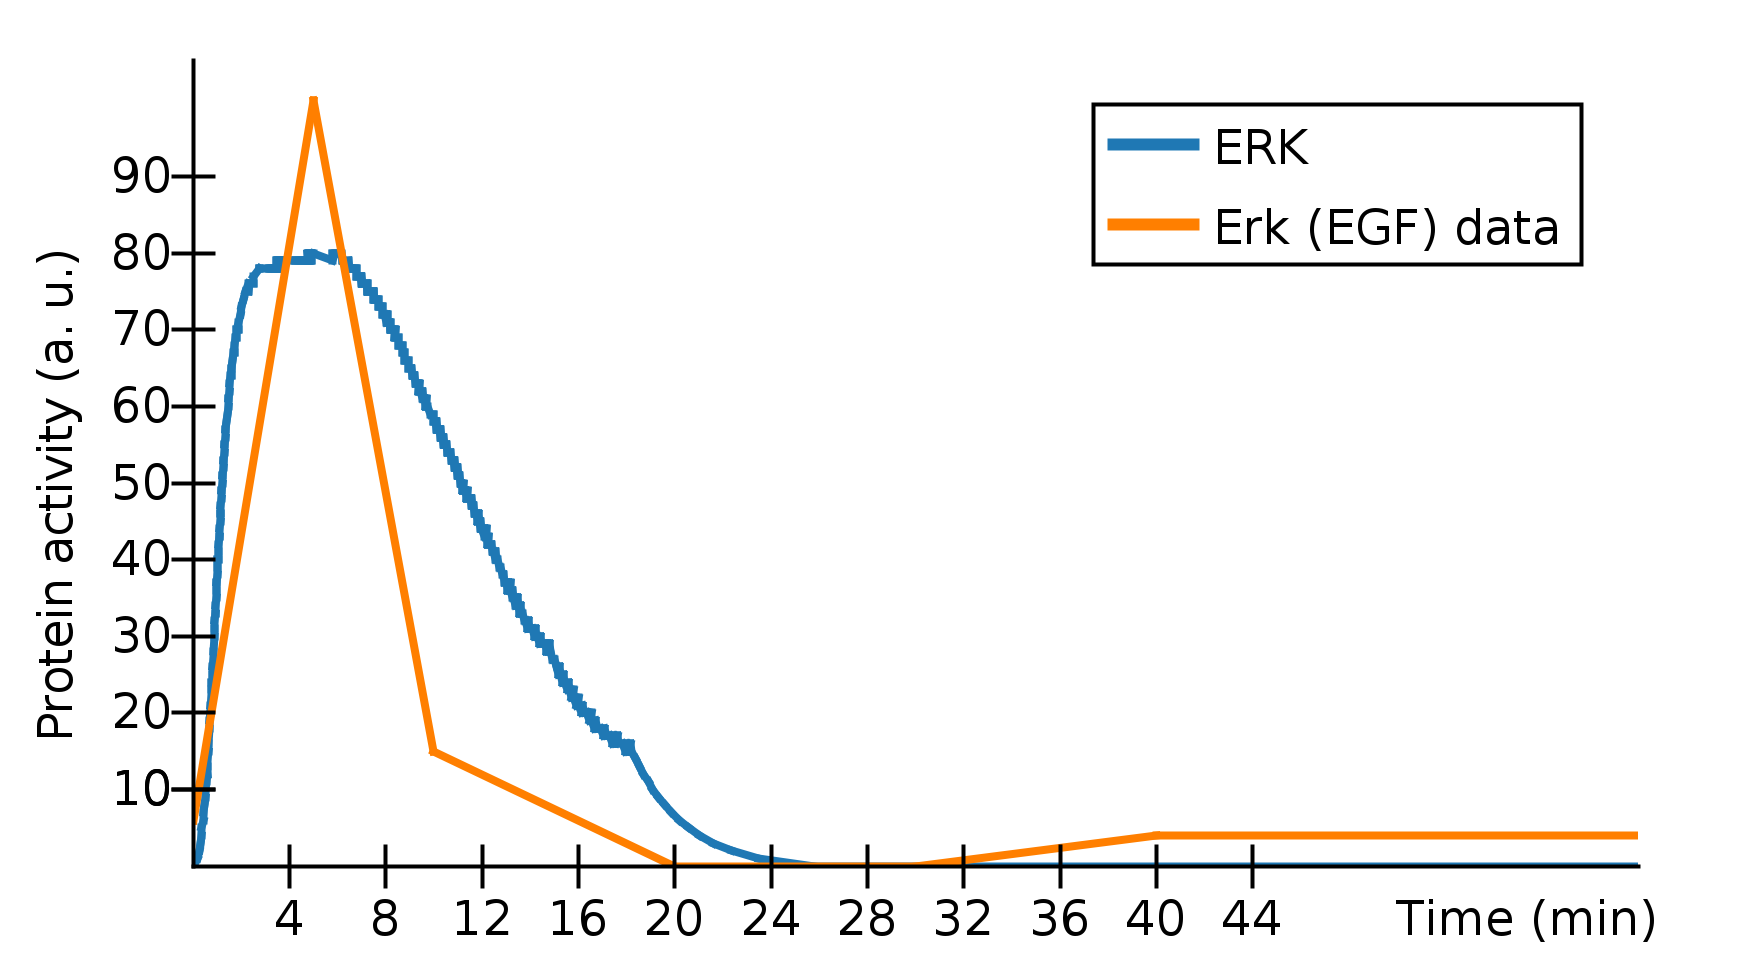
\includegraphics[width=.25\textwidth]{images/grafico_egf3}}%
\subfloat[\label{fig:ngf-graph}]{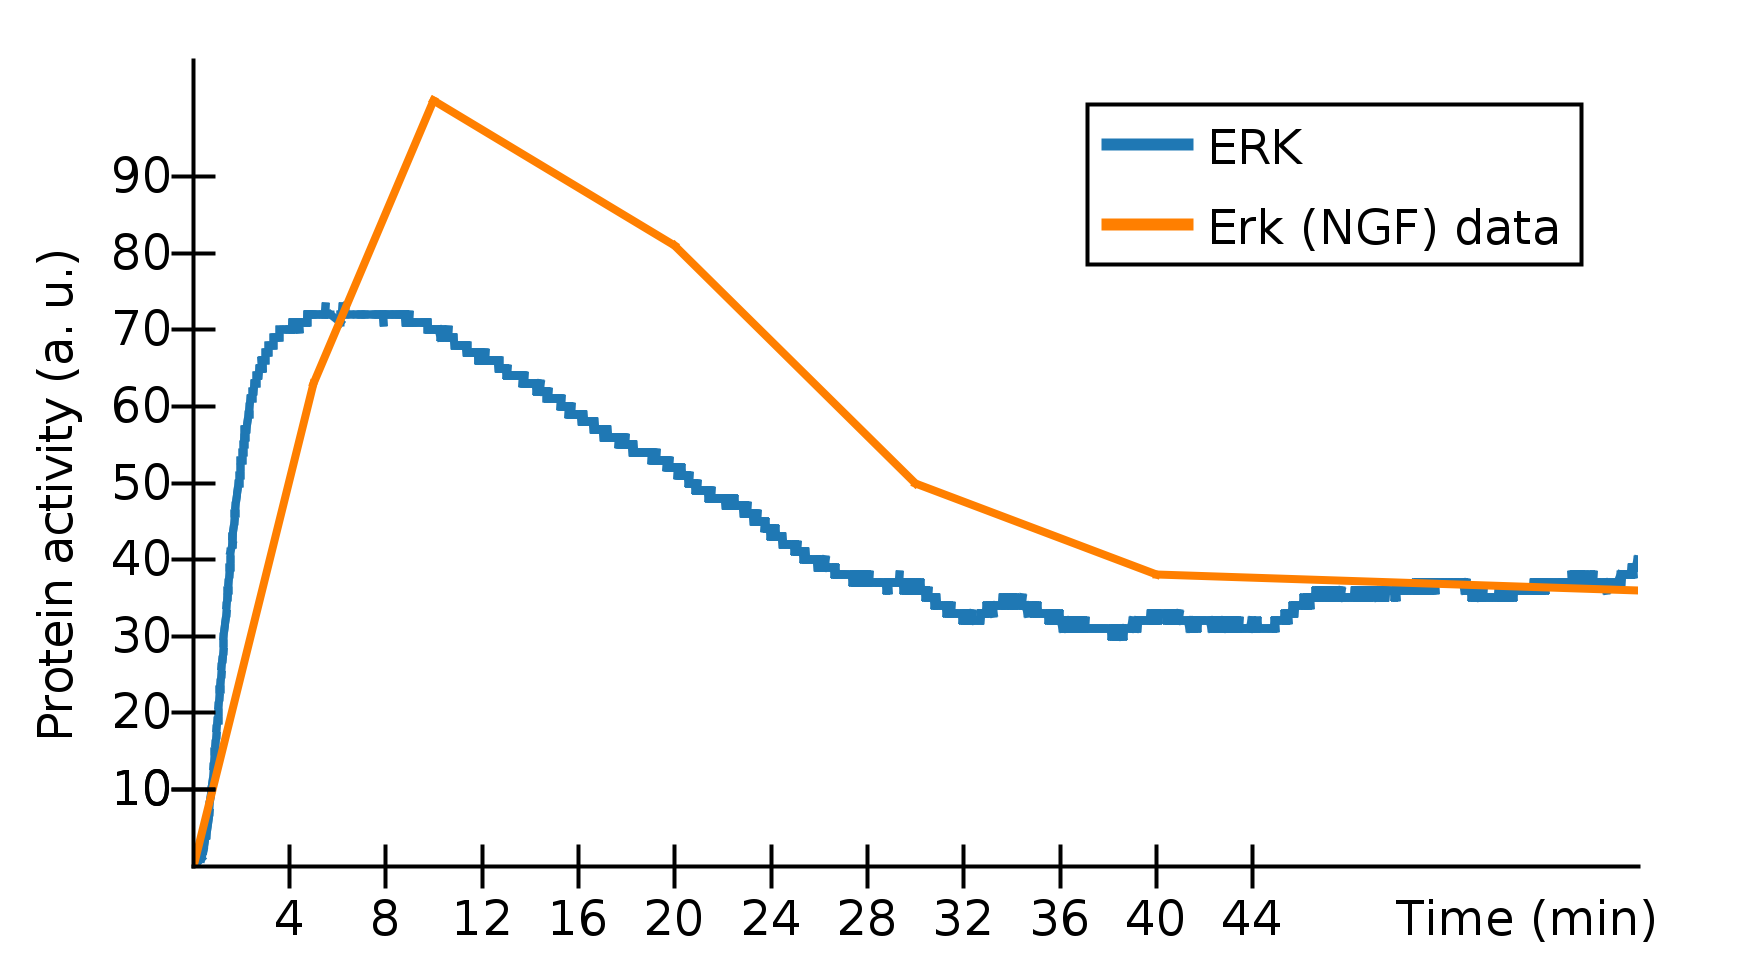
\includegraphics[width=.25\textwidth]{images/grafico_ngf3}}
\caption{Comparison of the model and experimental data.
{\bf \protect\subref{fig:egf-graph}}~Treatment with 100 ng/ml EGF results in transient ERK activation.
{\bf \protect\subref{fig:ngf-graph}}~Treatment with 50 ng/ml NGF results in sustained ERK activation.
The {\sf ERK} series are computed from the model, while {\sf Erk (EGF) data} and {\sf Erk (NGF) data}
are based on experimental data from Santos et al.~\cite{egf-ngf}.}
\label{fig:case-study-graphs}
\end{figure}


Due to a new addition to ANIMO, it is possible to highlight the differences in the network dynamics 
between two versions of the model. To this end, simulation results for one version of the model are subtracted from the results
of a second version. These differences are then visualized in the network topology, by using a suitable colour scheme. This allows a visual
evaluation of the influences of a change in the model on the resulting dynamic behaviour. Figure~\ref{fig:case-study-diff}
shows an example, with the differences in activities between 1) treatment with NGF and 2) treatment with EGF. It can be seen that 
a higher activity of PKC downstream of NGF leads to inhibition of RKIP, causing sustained ERK activity. 
This visualization can be used to rapidly assess the effect of model changes, such as extra nodes, 
different initializations, altered values for reaction parameters or a new wiring of the network. 
This feature is particularly useful when working with large models with extensive feedback loops, 
when the complete impact of changes to the model becomes much harder to grasp.

\begin{figure}[htb]
\centering
  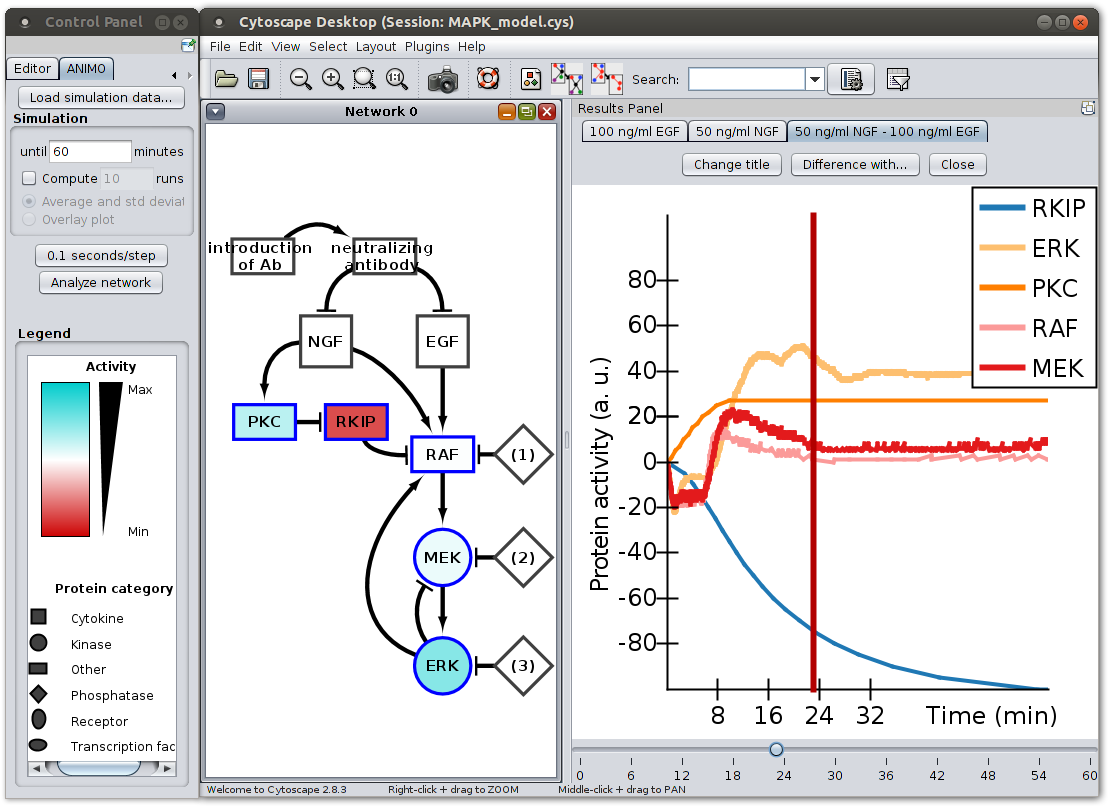
\includegraphics[width=.48\textwidth]{mapk_model_diff4}
\caption{Difference between the simulations obtained using
50 ng/ml NGF and 100 ng/ml EGF as input at 22 minutes (vertical red bar in right panel). In this mode, node colours
are based on the difference of activity between the two configurations of the model:
a green-coloured node is more active due to NGF treatment, while red indicates less activity and white
means no difference. Note that NGF and EGF are both white, since at 22 minutes, 
NGF and EGF are inactivated in both conditions by the neutralizing antibody. A slider underneath the graph can be used to 
interactively view the differences at different time points. \label{fig:case-study-diff}}
\end{figure}




\section{Related work}\label{sec:related-work}
Formal approaches to modelling biological systems can be divided into two large groups. The first 
includes approaches based on ordinary differential equations (ODEs), whereas the second 
encompasses methods based on concurrent systems. This distinction captures the main
characteristic of concurrent systems, which allows one to describe a system by specifying its
components in isolation, and then define the interaction rules. Methods based on ODEs on the other 
hand will need to explicitly account for all changes each interaction can cause to each component of the system.
Even if less maintainable, models based on ODEs are usually easier to understand, because of their strong
connection with the actual chemical reaction laws governing the evolution of a system. Approaches based 
on concurrency will usually add a layer on top of the canonical description of chemical reactions, 
requiring a user to acquire some practice before being able to fully benefit from the different paradigm.

Tools that allow to construct models based on ODEs include for example COPASI~\cite{copasi}, 
E-Cell~\cite{e-cell} and GNA~\cite{gna}.
These tools add to the potential of ODEs by coupling them with additional modelling approaches,
such as stochastic models\footnote{Stochastic modelling becomes particularly useful when some
molecular species have very small concentrations, which nullifies the assumption of a well-mixed solution used in models based on ODEs.}
used in COPASI and E-Cell, and by allowing for qualitative modelling, as does GNA.
Other tools, such as Systems Biology Workbench~\cite{sbw}, allow to couple high-performance
analysis engines (like roadRunner) to user-friendly interfaces (e.g. JDesigner). Finally, tools like CellDesigner~\cite{celldesigner}
provide an appealing graphical representation as an interface to powerful computational engines.
Most of the cited tools are founded on parameter-intensive approaches, while the paradigm implemented in ANIMO
uses less precise formulations, which requires less initial knowledge from the user.


Methods relying on concurrent systems
can be either qualitative or quantitative. The distinction is based on the possibility to add numerical 
(quantitative) information to the model, such as reaction rates, molecular concentrations, and reaction volumes. 
ANIMO is a quantitative method based on concurrent systems. 
The use of \tas\ to model biological signalling events has been described before by Maler and Batt~\cite{oded-ta-discretization}. 
ANIMO takes a less general approach, tailored for the construction of more abstract models.


\section{Conclusions and future work}\label{sec:conclusions}
We contribute to the modelling of biological pathways by introducing a formalization of the
domain-specific language traditionally used for pathway representations into a model based on Timed Automata (\tas).
The ANIMO user interface makes the power of \tas\ available 
to users that lack a thorough background in mathematics or computer science. This will likely contribute to to the 
dissemination of computational modelling in the realm of molecular cell biology and regenerative medicine.
In this respect, we are applying ANIMO in a research project aimed at studying
chondrocyte signalling in relation to osteoarthritis~\cite{oa-bio1,oa-bio2}. The objective is to enhance
cartilage tissue engineering strategies by investigating the effect of
extracellular signalling molecules and cell-matrix interactions in order to mimic
these signals in the development of biomaterials that provide direct
support, while stimulating chondrocytes to repair the damaged cartilage tissue.

The use of \tas\ as the underlying formalism of ANIMO lies the foundation to the use of more advanced 
analysis techniques to query constructed models. In particular, applying model checking techniques would allow us to perform \emph{in silico} experiments, answering questions
such as ``What is the combination of inputs that leads to $\mbox{activity}(A) \geq 20/50$
and $\mbox{activity}(B) < 10/80$ in 120 minutes?''. Moreover, taking advantage of statistical model
checking capabilities recently introduced to UPPAAL~\cite{uppaal-smc}, we plan to extend the current modelling paradigm adding the possibility
to define stochastic behaviour (e.g., assign an exponential distribution to the addition of a drug as input to the network),
and support probabilistic queries such as ``What is the probability that
$\mbox{activity}(A) \geq 40/50$ in 30 minutes?''.
Other interesting developments are aimed at further speeding up the modelling phase, in order to let the user
start interrogating a model as soon as possible. We plan to include a support for parameter
sensitivity analysis and automated parameter fitting to a given experimental data set. 
After having defined a measure of distance between the model and the experimental data, we plan to minimize that distance
via (user-defined) parameter sweeps.
We are also developing
techniques based on automata learning~\cite{test-based-modelling} for deriving the topology of a biological network, based
on a series of constraints and experimental data series.

In the future, ANIMO and related tools may lead to a new paradigm for interactive representation of
biological networks. Networks in digital textbooks and articles could be displayed as animations amenable to
modifications by readers. Repositories of formal descriptions of signalling modules could be used to put together
executable signalling networks. In general, the process of formalizing biological knowledge will lead
to a more thorough understanding of biological networks and will accelerate hypothesis-driven research.

\bibliographystyle{IEEEtran}
\bibliography{Paper}



\end{document}


